\chapter{Camima: a multi-camera and image process platform}
\label{chap:camima}

% What is Camima and why we need to develop it?
Camima is multi-camera control platform with image processing functions. Thanks to various camera adaptors provided by Image Acquisition Toolbox, Camima can support varioius camera type, including USB cameara from PointGrey, PCO and Migtex, Web camera and other general type of cameras. The main time sequence is tailered for the absoption image for cold atom experiment. After acquizting images from camera, there are extendable and programable image processing functions for post-process images. Users can easily re-program the time squence and processing sequence for various seneros, e.g. denoising or defringe process, flourencense image and so on.

The software is made of four parts: Camima: main control for converting data from different camera to a uniform image stream, which easier for following processing. Vuima: for showing and processing images. Camset: a general setting program for various camera. Fitset: for general purpose fitting progress.

\section{licensing, versions and updates}
% licensing
This programs is a free software: you can redistribute them and/or modify them under the terms of the GNU General Public License, version 3, as published by the Free Software Foundation. The full text of the license is available from \href{https://www.gnu.org/licenses/}{https://www.gnu.org/licenses/} and is included in the file COPYING included in the distribution.

% Version control
For adapting different version of MATLAB and its Appdesigner toolbox, this program is created with the following versions:
\begin{itemize}
\item MATLAB2016
\item MATLAB2020
\end{itemize}

% download and updates
Software downloads and updates are made available via github:
\begin{itemize}
\item \href{https://github.com/guozc12/Camima}{https://github.com/guozc12/Camima}
\end{itemize}

\section{Using the software: a basic guide}
\subsection{Prerequisites}
Before install Camima, MATLAB with version later than 2016 is needed. The listed several add-ons are needed.
\begin{itemize}
    \item MATLAB
    \item Appdesigner™ in MATLAB
    \item Image Acquisition Toolbox™ in MATLAB
    \item uitree in MATLAB
\end{itemize}

\subsection{Start Camima}
% add Camima_main, i.e. main interface (done: 2021年8月4日21:43:37)
\begin{figure}[htb]
\begin{center}
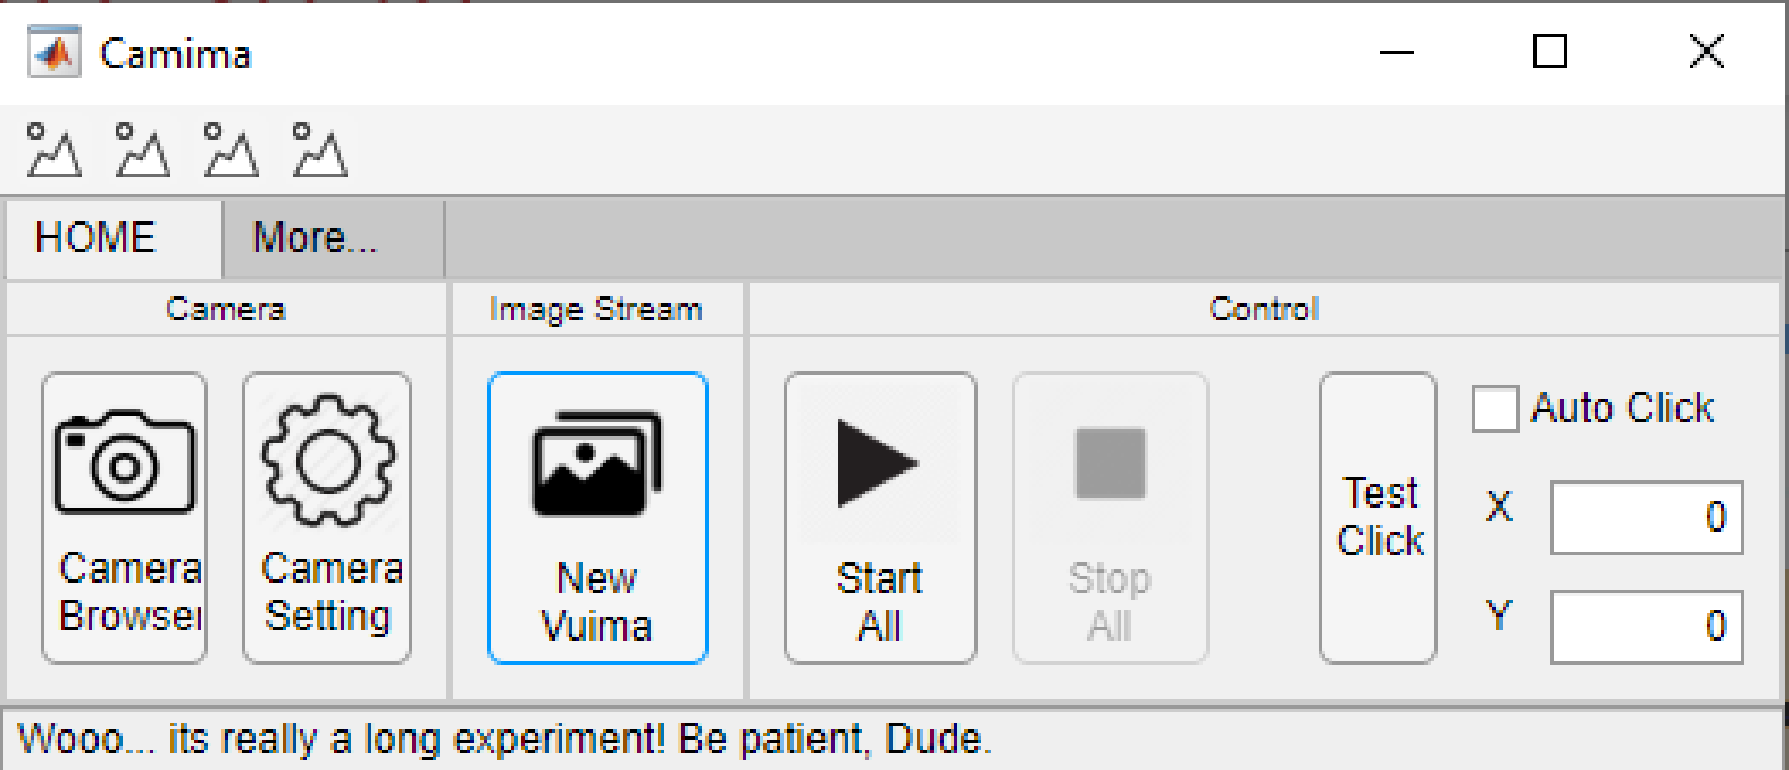
\includegraphics [width = 0.8 \linewidth]{Camima_main.pdf}
\end{center}
\caption{}
\label{Camima_main}
\end{figure}

% introducing the main panel (done: 2021年8月4日21:43:48)
Open the Camima.mlpp in Appdesigner. Then Click the Run button to run the main Camima program. As shown in Fig. \ref{Camima_main}, a small panel show you entrances for different functions:
\begin{itemize}
    \item Camera Browser: Open a new panel for searching and initializing all installed cameras. (As shown in Fig. \ref{Camima_CamTree})
    \item Camera Setting: Open a new panel (Camset) for control each camera directly.
    \item New Vuima: Open a image processing panel (Vuima) for viewing images and automatic image processing.
    \item Start All: For quick starting everything, including start acquizition for every camera
    \item Stop All: For quick stopping everything.
    \item Test Click: for setting a button click after each shot with the written position on right side.
\end{itemize}

% add Camima_CamTree, i.e. Camera browser
\begin{figure}[htb]
\begin{center}
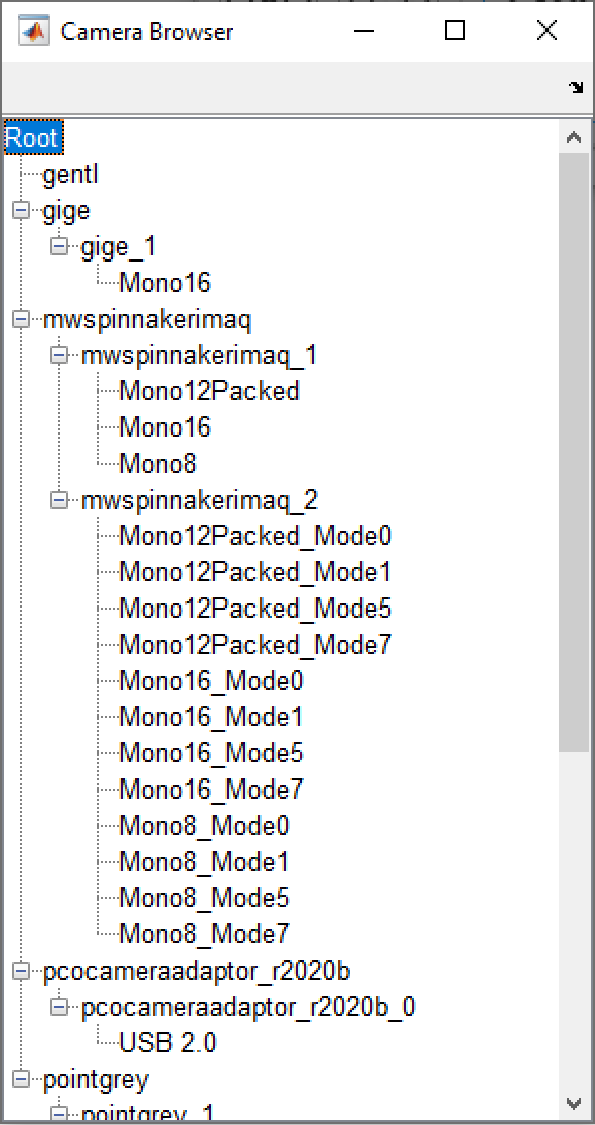
\includegraphics [width = 0.4 \linewidth]{Camima_CamTree.pdf}
\end{center}
\caption{}
\label{Camima_CamTree}
\end{figure}

\subsection{camera setting}
% camera adaptors for different venders

\begin{itemize}
    \item PointGrey
    \item BlackFly
    \item PCO camera
    \item Web Cam
    \item ...
\end{itemize}

% Control
As shown in Fig. \ref{Camima_Camset}, after catching each camera, we can control the camera manually, such as previewing, manual trigger for acquisition. For cameras from different vendors, the general settings are different. Thus, we generate a list in a new window, as shown in right panel of Fig. \ref{Camima_Camset}. User can change properties of camera, such as exposure time and binning. The ROI (Region-of-interest) can be set when camera is stop. More setting about automatic trigger can be set in the right-bottom panel of Camset window.

% add Camima_Camset, i.e. Camera setting
\begin{figure}[htb]
\begin{center}
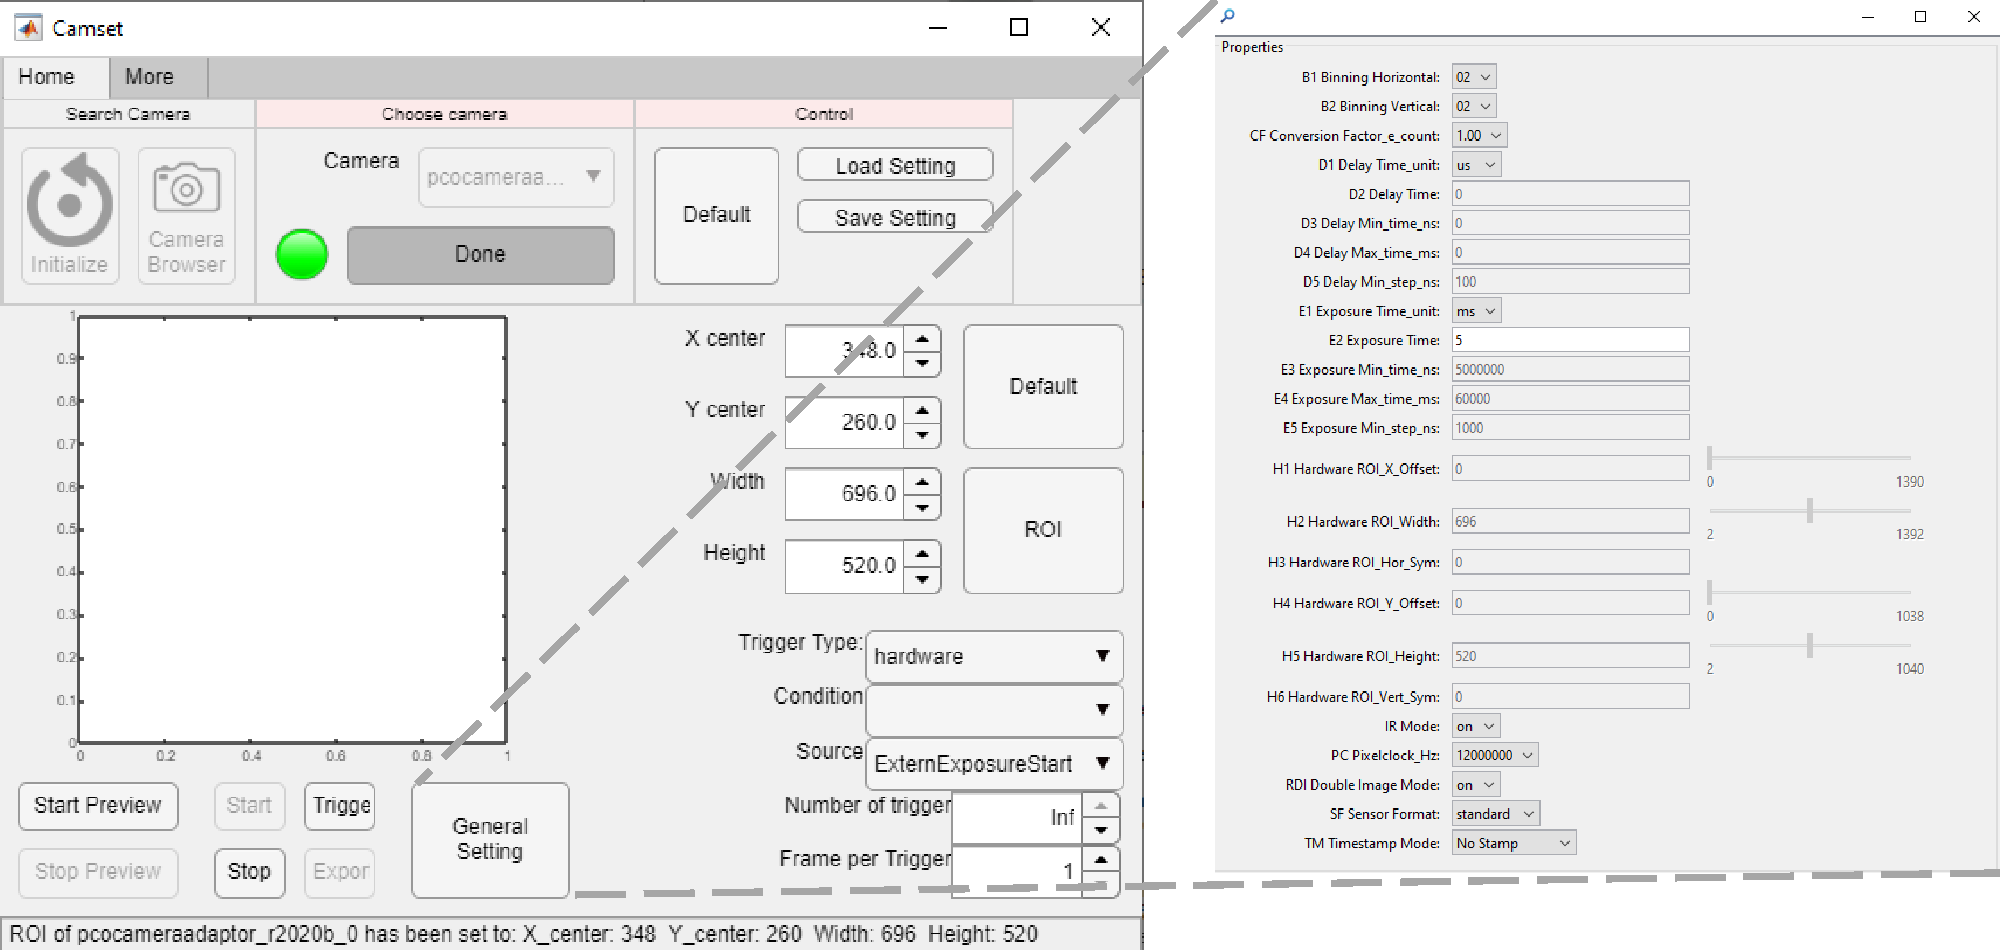
\includegraphics [width = \linewidth]{Camima_Camset.pdf}
\end{center}
\caption{}
\label{Camima_Camset}
\end{figure}

\subsection{Image acquisition}


% add Camima_Vuima, i.e. Viewing the image
\begin{figure}[htb]
\begin{center}
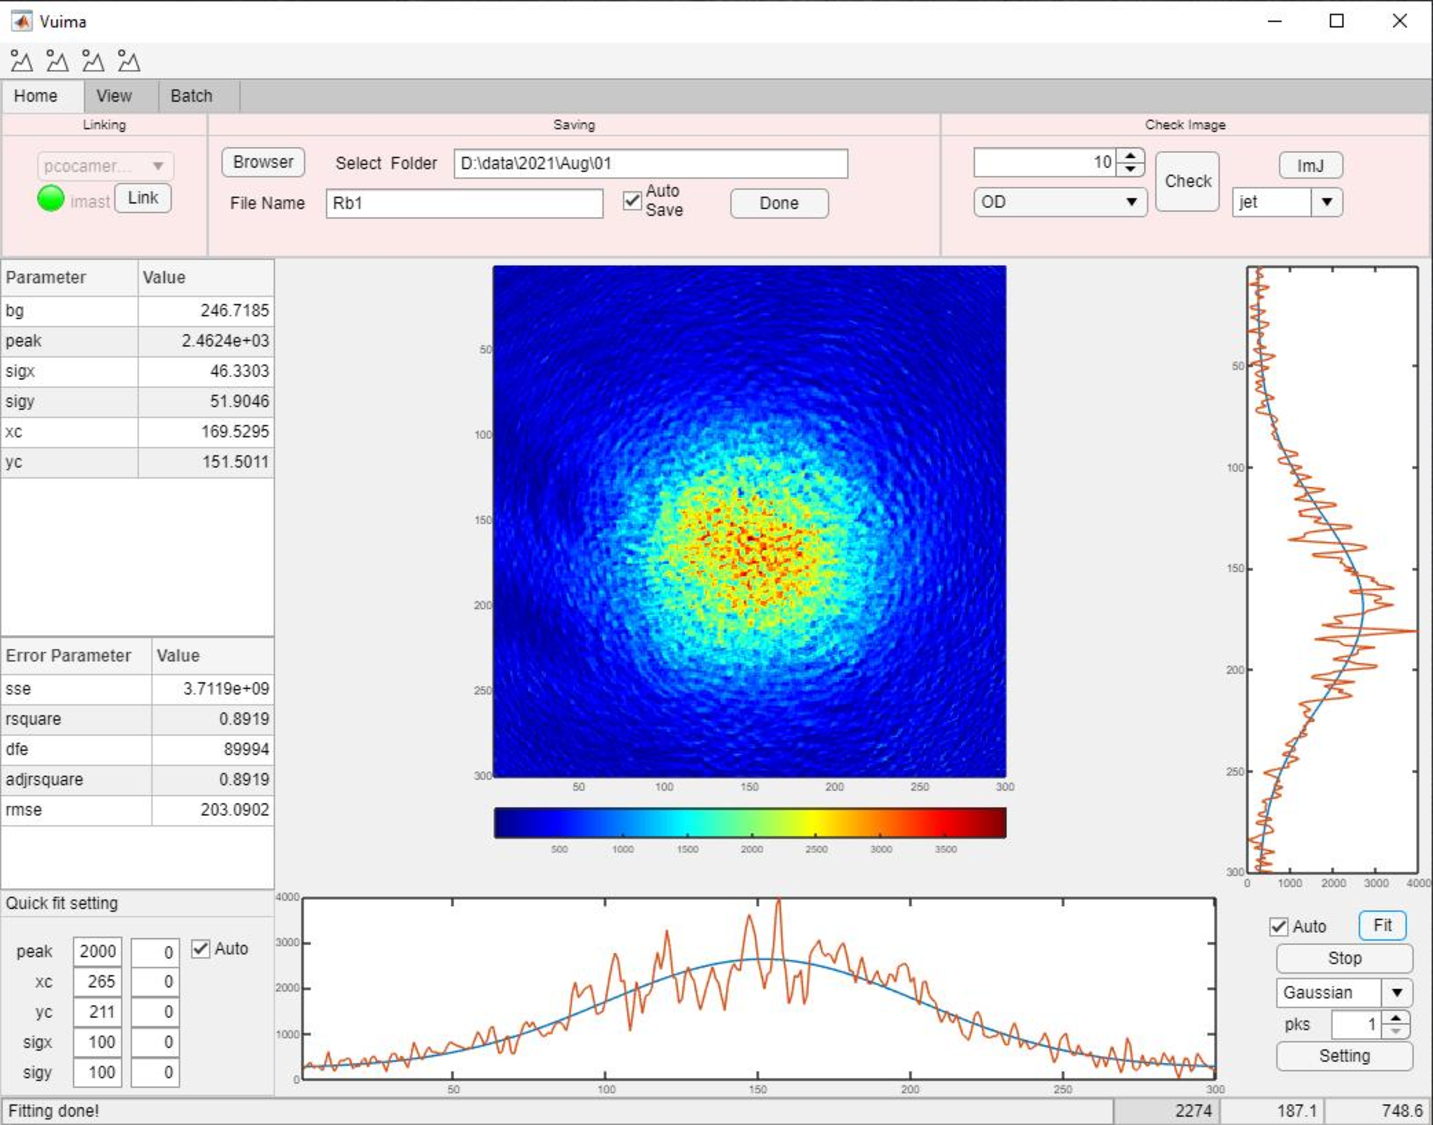
\includegraphics [width = \linewidth]{Camima_Vuima.pdf}
\end{center}
\caption{}
\label{Camima_Vuima}
\end{figure}

1. time sequence of image axquisition
2. converting camera data to image stream
3. show and pre-process of images on Vuima

\subsection{post precessing of image}

% add Camima_Fitset, i.e. Setting the fitting
\begin{figure}[htb]
\begin{center}
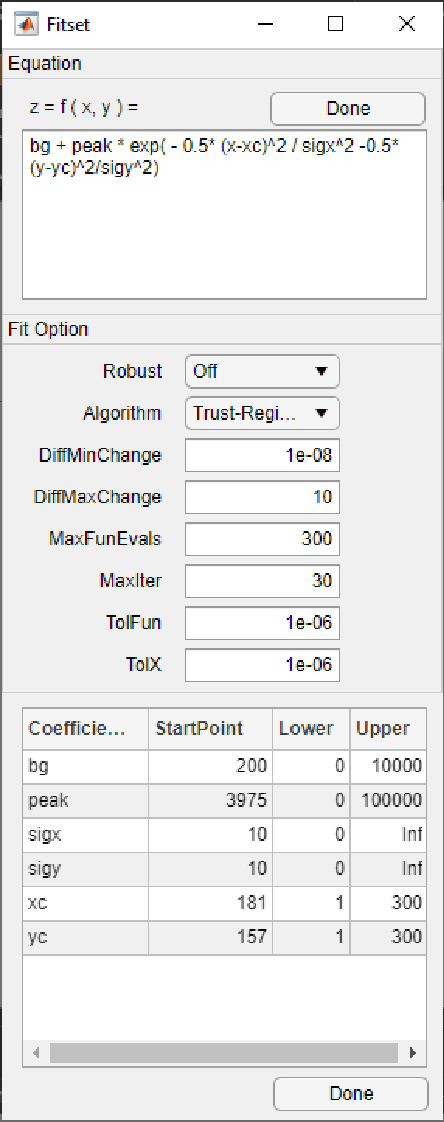
\includegraphics [width = 0.4\linewidth]{Camima_Fitset.pdf}
\end{center}
\caption{Camima-Fitset: }
\label{Camima_Fitset}
\end{figure}

1. statistic data from image
2. fitting of image
3. batch processing

\chapterend

